The points of trisection are
 \begin{align}
\vec{C} &= \frac{0.5\vec{A}+\vec{B}}{0.5+1} \\
\vec{D} &= \frac{2\vec{A}+\vec{B}}{2+1}\\
\implies \therefore \vec{C} &= \myvec{0\\-2.33},
\vec{D} = \myvec{2\\-1.66}
\end{align}
The following Python code generates Fig. \ref{fig:3.6.2_trisection_pts_on_a_line}
\begin{lstlisting}
solutions/2/codes/line_ex/pts_on_a_line/trisection.py
\end{lstlisting}

\begin{figure}[!ht]
\centering
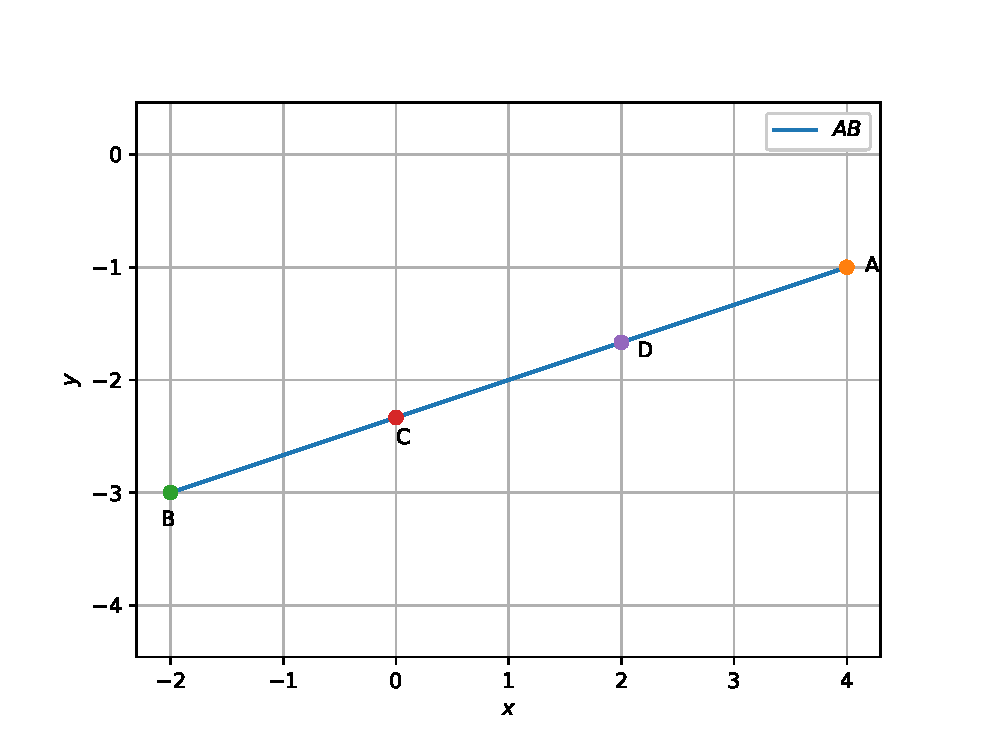
\includegraphics[width=\columnwidth]{./solutions/2/figs/line_ex/pts_on_a_line/trisection.eps}
\caption{}
\label{fig:3.6.2_trisection_pts_on_a_line}
\end{figure} 


